\documentclass[11pt]{article}

\usepackage{amsmath, amsthm, amssymb, graphicx, psfrag, dcolumn, bm, accents, textcomp, hyperref, url}
\usepackage{graphicx,psfrag,textcomp,amsmath,amsthm,amssymb,fancyhdr,fancybox}
\usepackage{setspace,url,color,wasysym,pstricks,multirow,rotating}

\setlength{ \topmargin}{-.5in} \setlength{ \oddsidemargin} {-.4in}
\setlength{ \evensidemargin} {-.4in}
\setlength{ \textwidth} {6.5in}
\setlength{ \textheight} {9.0 in}

\usepackage{ifthen}
\newboolean{solutions}
\setboolean{solutions}{false}

\newcommand{\sols}[2]{\ifthenelse{\boolean{solutions}}{\small\emph{#1}\normalsize}{#2}}
\usepackage{tikz}
\usetikzlibrary{arrows}
\usetikzlibrary{shapes}
\usetikzlibrary{positioning}
\tikzstyle{block}=[draw opacity=0.7,line width=1.4cm]

%% 
%% Custom colors...
%%
%\newrgbcolor{lightblue}{0. 0. 0.80}
%\newrgbcolor{white}{1. 1. 1.}
%\newrgbcolor{whiteblue}{.80 .80 1.}
%\newrgbcolor{crimson}{0.6 0.00 0.20}
%\newrgbcolor{lightcrimson}{0.6 0. 0.1}
%\newrgbcolor{whitecrimson}{1. 0.8 0.8}
%\newrgbcolor{indigo}{0.33 0. 0.49}

%\renewcommand{\labelenumi}{(r\oman{enumi})}
%\renewcommand{\labelenumii}{(\alph{enumii})}
\renewcommand{\theenumi}{\arabic{enumi}}
\renewcommand{\theenumii}{\alph{enumii}}
\renewcommand{\labelenumi}{\bf \theenumi.}
\renewcommand{\labelenumii}{\bf (\theenumii)}

\def\Pr{\mathbb{P}}

\newenvironment{questions}{\begin{enumerate}}{\end{enumerate}}

%%%%%%%%%%%%%%%%%%%%%%%%%%%%%%%%%%%%%%%%%%%%%%%%%%%%%
\def\hwknumber{1}
%%%%%%%%%%%%%%%%%%%%%%%%%%%%%%%%%%%%%%%%%%%%%%%%%%%%%

\begin{document}

\textbf{Homework 1 Solutions: Bayesian Inference Module}

\begin{flushright}
 STA 250 Fall 2013, Prof. Baines (10/26/13)
\end{flushright}

\begin{itemize}

 \item[Q1] Under the assumption that the resulting Markov Chain is ergodic (i.e., aperiodic and positive recurrent) with continuous state space, we know that the chain converges to a stationary distribution $\pi$ satisfying:
 \begin{align}\label{stat_cond}
 \pi(y) = \int{}\pi(x)\mathcal{P}(x,y)dx  
 \end{align}
 Therefore, we must show that for $\mathcal{P}$ corresponding to a Gibbs sampler, the target density $\pi$ satisfies equation~\eqref{stat_cond}. If we can show this, then we have shown that the target density is the stationary distibution for the Gibbs sampler. Note that the stationary distribution can be seen to be unique under certain regularity conditions. For a two-dimensional Gibbs sampler, the states are $x=(x_{1},x_{2})$ and $y=(y_{1},y_{2})$ with the transition density given by:
 \begin{align*}
 \mathcal{P}(x,y) = \pi_{1|2}(y_{1}|x_{2})\pi_{2|1}(y_{2}|y_{1}) ,
 \end{align*}
 where $\pi_{1|2}$ and $\pi_{2|1}$ are the conditional distributions defined by the joint target density $\pi$. For brevity we drop the subscripts on $\pi$ as the conditional densities are clear from the context. Therefore, we see that:
 \begin{align*}
 \int{}\pi(x)\mathcal{P}(x,y)dx  &= \int{}\pi(x_{1},x_{2})\pi(y_{1}|x_{2})\pi(y_{2}|y_{1})dx_{1}dx_{2} \\
                                 &= \int{}\pi(x_{2})\pi(y_{1}|x_{2})\pi(y_{2}|y_{1})dx_{2} \\ 
                                 &= \int{}\pi(y_{1},x_{2})\pi(y_{2}|y_{1})dx_{2} \\ 
                                 &= \pi(y_{1})\pi(y_{2}|y_{1}) = \pi(y_{1},y_{2}) .
 \end{align*}
Therefore the target density $\pi$ is seen to be the stationary distribution of the chain.\\
$ $\\
For a $p-$dimensional (sequential) Gibbs sampler we just extend the result slightly. The transition density becomes:
 \begin{align*}
 \mathcal{P}(x,y) = \prod_{j=1}^{p}\pi(y_{j}|y_{[1:j-1]},x_{[(j+1):p]}) ,
 \end{align*}
 where $y_{[1:0]}:=\varnothing$. Therefore, we see that:
 \begin{align*}
 \int{}\pi(x)\mathcal{P}(x,y)dx  &= \int{}\pi(x_{1},\ldots,x_{p})\prod_{j=1}^{p}\pi(y_{j}|y_{[1:j-1]},x_{[(j+1):p]}) dx_{1}\cdots{}dx_{p} \\
                                 &= \int{}\pi(x_{2},\ldots,x_{p})\prod_{j=1}^{p}\pi(y_{j}|y_{[1:j-1]},x_{[(j+1):p]}) dx_{2}\cdots{}dx_{p} \\ 
                                 &= \int{}\pi(y_{1},x_{2},\ldots,x_{p})\prod_{j=2}^{p}\pi(y_{j}|y_{[1:j-1]},x_{[(j+1):p]}) dx_{2}\cdots{}dx_{p} \\ 
                                 &= \int{}\pi(y_{1},x_{3},\ldots,x_{p})\prod_{j=2}^{p}\pi(y_{j}|y_{[1:j-1]},x_{[(j+1):p]}) dx_{3}\cdots{}dx_{p} \\ 
                                 &= \int{}\pi(y_{1},y_{2},x_{3},\ldots,x_{p})\prod_{j=3}^{p}\pi(y_{j}|y_{[1:j-1]},x_{[(j+1):p]}) dx_{3}\cdots{}dx_{p} \\ 
                                 &= \cdots \\
                                 &= \pi(y_{1},y_{2},\ldots,y_{p}) ,
 \end{align*}
 as needed. A little bit more elegantly, let:
  \begin{align*}
  Q_{k} = \pi(y_{[1:(k-1)]},x_{[k:p]})\prod_{j=k}^{p}\pi(y_{j}|y_{[1:(j-1)]},x_{[(j+1):p]})
 \end{align*}
 Then it can be seen that:
  \begin{align*}
  \int{} Q_{k} dx_{k} &= \pi(y_{[1:k]},x_{[(k+1):p]})\prod_{j=k+1}^{p}\pi(y_{j}|y_{[1:(j-1)]},x_{[(j+1):p]}) = Q_{k+1} , \qquad k=1,\ldots,p-1, \\
  \int{} Q_{p} dx_{p} &= \pi(y_{[1:p]}) .
 \end{align*}
 This gives us:
 \begin{align*}
 \int{}\pi(x)\mathcal{P}(x,y)dx  &= \int{}Q_{1}dx_{1}\cdots{}dx_{p} = \int{}Q_{2}dx_{2}\cdots{}dx_{p} = \cdots = \int{}Q_{p}dx_{p} = \pi(y) .
 \end{align*}
 
 \item[Q2] The two main algorithms most people implemented here were a multivariate Metropolis algorithm (with a Normal random walk proposal) and a Metropolis-within-Gibbs algorithm (again, using Normal random walk proposals). Most coverage plots looked something like Figure~\ref{cp}.
 
 \begin{figure}[h]
 \begin{center}
  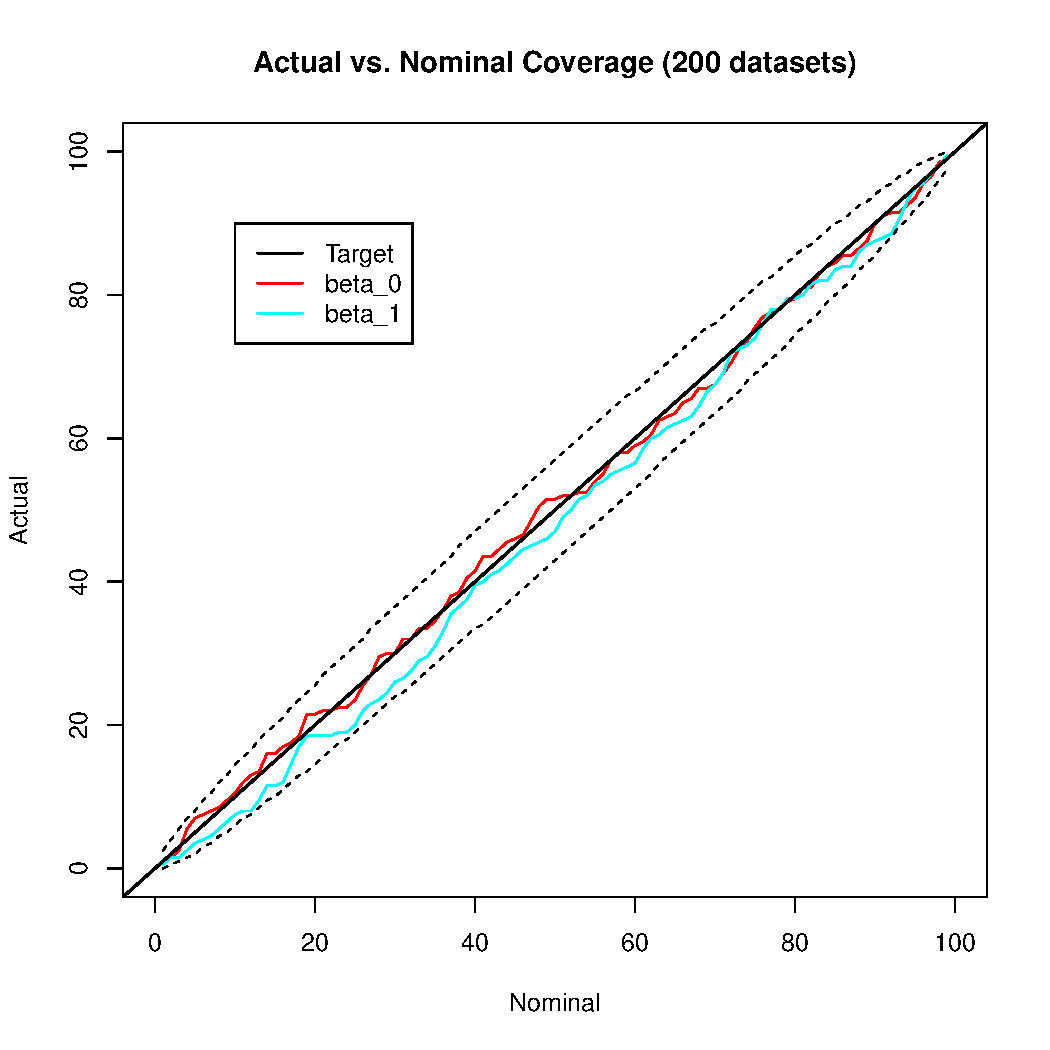
\includegraphics[scale=0.5]{coverage_line_plot.pdf}
  \caption{Coverage plot for Q2}\label{cp}
 \end{center}
 \end{figure}
 
 \item[Q3] There were differing degrees of success in tackling this problem. The course GitHub repo has solution code for those who couldn't get things to run. A couple of notes:
 \begin{itemize}
 \item Run more iterations! Unless computing time is a big issue, run for more iterations than you need. For example, set the number of iterations to 500k and leave things to run on Gauss (unless your code was very inefficient this shouldn't take too long. For example, my code takes 9 minutes to run 500k iterations on an old laptop). 
 \item Using \texttt{mcmc} objects from \texttt{library(coda)} (when using \texttt{R}) makes life much simpler.
 \item Covariance matrices for the proposal distribution needed to be selected carefully. Most successful choices were based on the covariance matrix from a regular \texttt{lm} or \texttt{glm} fit to the data.
 \end{itemize}
 
 Example traceplots are given in Figure~\ref{tp}.
 
 \begin{figure}[h]
 \begin{center}
  \includegraphics[scale=0.5]{bc_posteriors_MH__02.png}
  \caption{Traceplots for Q3 (unstandardized)}\label{tp}
 \end{center}
 \end{figure} 
 
 Posterior estimates for the standardized and non-standardized cases are given below.
 \begin{verbatim}
  
  Unstandardized Results:
  =====================
                  2.5%       25%       50%      75%    97.5%
Intercept   -33.646603 -19.97332 -13.37311 -6.97462  4.56086
area          0.002933   0.02297   0.03339  0.04341  0.06282
compactness -31.961992 -13.29931  -3.53277  6.12656 24.34174
concavepts   22.091979  46.37750  59.29670 72.32769 97.64969
concavity    -5.033865   3.65120   8.17016 12.83947 22.23377
fracdim     -67.036530 -29.34780  -9.68547  9.80690 47.50416
perimeter    -0.949401  -0.36876  -0.06827  0.22715  0.81614
radius       -8.038762  -3.58885  -1.38465  0.86469  5.11523
smoothness   13.793833  39.65263  53.44324 67.38485 94.48697
symmetry     -2.035344  11.20961  17.95906 24.70283 37.49552
texture       0.255499   0.32747   0.36717  0.40900  0.49198
  
  
  Standardized Results:
  =====================  
                2.5%      25%     50%      75%   97.5%
Intercept    -0.7355   0.0267  0.4389  0.81986  1.5809
area          1.9959   9.6230 13.8054 18.13752 26.2322
compactness  -2.2540  -0.8715 -0.1518  0.58897  2.0037
concavepts    0.5985   2.0095  2.7577  3.55913  5.2764
concavity    -0.5620   0.3531  0.8288  1.28917  2.1910
fracdim      -1.7799  -0.9534 -0.5175 -0.09353  0.7399
perimeter   -24.7027  -9.6716 -2.0238  5.48899 19.7902
radius      -29.5539 -14.5519 -6.5121  1.50326 17.3198
smoothness    0.2732   0.8634  1.1713  1.48762  2.1227
symmetry     -0.1017   0.2856  0.4901  0.69491  1.1048
texture       1.2646   1.6107  1.8069  2.01321  2.4510
 \end{verbatim}

 The posterior predictive distribution for the mean (i.e., proportion of 1's) are shown in Figure~\ref{ppc} for the unstandardized setting.
 Note that other predictive statistics that aggregate over observations without accounting for the $x_{i}$'s do not
 provide additional information beyond the mean.

 \begin{figure}[h]
 \begin{center}
  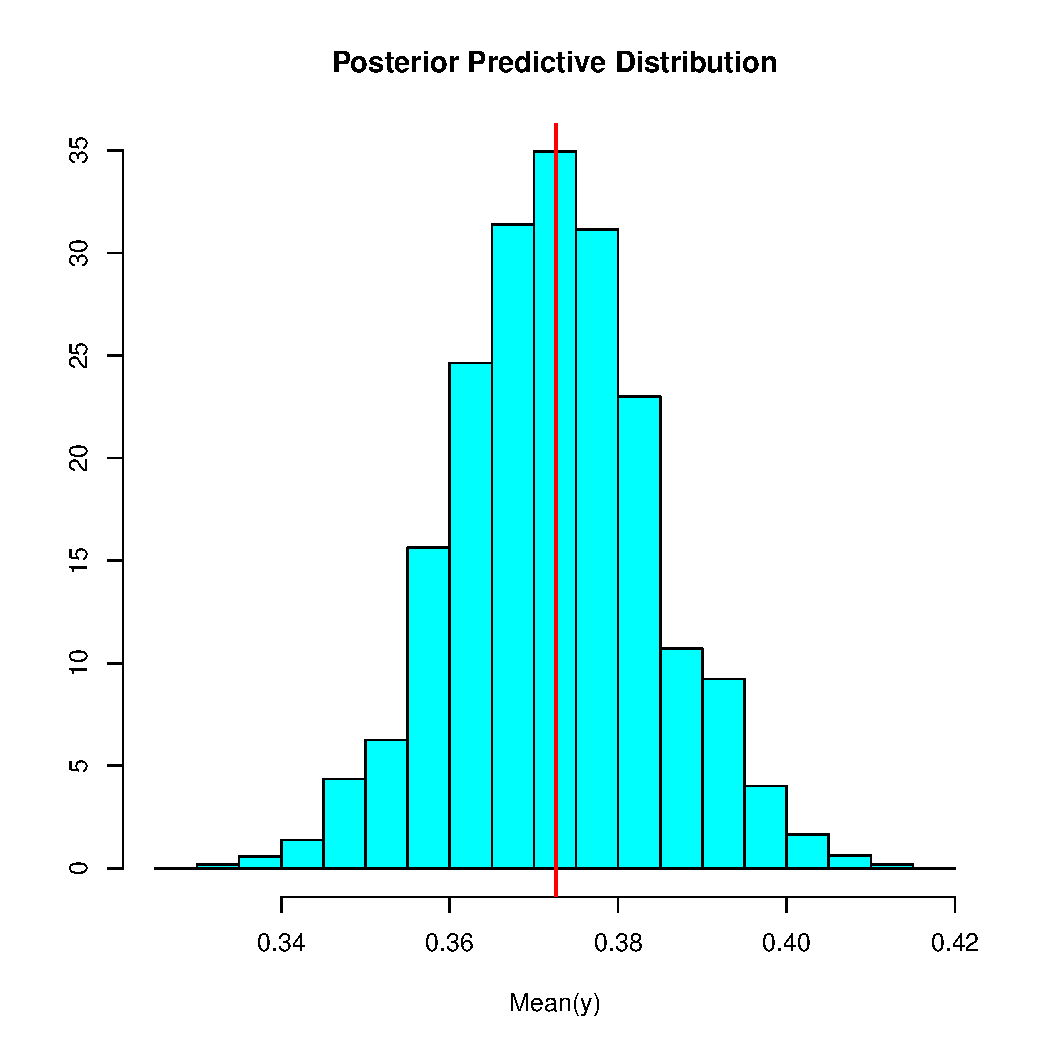
\includegraphics[scale=0.5]{bc_ppc.pdf}
  \caption{Posterior predictive distribution of proportion of 1's in the dataset (unstandardized)}\label{ppc}
 \end{center}
 \end{figure}
 
 
\end{itemize}


\end{document}
